\documentclass{article}
\usepackage[catalan]{babel}
\usepackage[utf8]{inputenc}
\usepackage{graphicx}
\usepackage{wrapfig}
\usepackage{amsmath}
\usepackage{amssymb}
\usepackage{ragged2e} 
\usepackage{subfig}
\usepackage{caption}
\usepackage{subcaption}
\usepackage[usenames]{color}
\usepackage{xcolor}
\usepackage{float}
\usepackage{chngcntr}
\usepackage{ragged2e}
\usepackage{multirow}
\usepackage{multicol}
\usepackage{vmargin}
\usepackage{hyperref}
\usepackage{subfigure}
\usepackage{url}

\begin{document}

\begin{titlepage}
    \centering
    \vspace{4cm}
    {\bfseries\LARGE Universitat Autònoma de Barcelona\newline Facultat de Ciències\par}
    \vspace{6cm}
    {\scshape\Huge Practice 1: \par Linear Regression Model \par}} 
    \vspace{2cm}
    {\Large \itshape Autors: \par}
    {\Large Andrea Gonzalez \& Gerard Lahuerta\par}
    {\small NIU: 1603921, 1601350\par}
    \vspace{3cm}
    {\Large 3 de Març del 2022\par}
\end{titlepage}

\justifying
\newpage
\setcounter{page}{2}
\pagestyle{plain}
\tableofcontents
\cleardoublepage
\addcontentsline{}{chapter}{}


\section{First Exercice}
\begin{itemize}
    \item \textbf{Statement:}\\ 
Perform a multiple linear regression with selling price as the response and
all the other variables except brand as the predictors. Write out the model
in equation form and indicate the design matrix. Provide an interpretation
of each coefficient in the model. Comment on the output of \texttt{summary()} function.
    \item \textbf{Perfom of the linear regression:} \\
Firstly, we have to obtain the data from our database (in this case a document excel).
\begin{verbatim}
install.packages("readxl")
library("readxl")

data = read_excel('~/Descargas/cars.xlsx')
\end{verbatim}
To perfom the multiple linear regression, we used the R function \texttt{lm()} which arguments we are using are the formula (the one that we want to obtain) and the data. \\ 
(\textit{There are much more arguments but we do not have to use them all.})
    \begin{verbatim}
linear_regression = lm( data$selling_price ~ data$year + data$fuel + 
                        data$seller_type + data$transmission + data$owner + 
                        data$km_driven, data )
    \end{verbatim}
The code above returns all the information of the multiple linear regression. \\\\
To obtain the coefficients of the multiple linear regression, we used the function \texttt{coef()} with the parameter the structure multiple linear regresion.
    \begin{verbatim}
coef(linear_regression)
    \end{verbatim}
Moreover, if we want to obtain the design matrix, we just have to use the \texttt{model.matrix()} expression.
    \begin{verbatim}
model.matrix(linear_regression)
    \end{verbatim}
    \item \textbf{Interpretation of the coefficient:} \\
    The function explained before (\texttt{coef()}), returns (in this case) the following output:
    \begin{verbatim}
(Intercept)                     data$year 
 -8.961922e+04                   4.528498e+01 
data$fuelElectric               data$fuelLPG 
 -8.259075e+02                   -2.891930e+02 
data$fuelPetrol                 data$seller_typeIndividual 
 -2.851035e+02                   -3.790299e+01 
data$transmissionManual         data$ownerSecond & Above Owner 
 -8.720734e+02                   -3.624312e+01 
data$km_driven 
 -8.111749e-01 
    \end{verbatim}
We can clearly see a difference between the coefficients (ones are positive whereas the others are negative). This means that the selling price increases depending on some aspects or decreases depending  in others (what seems logical).\\
Moreover, if its absolute value is bigger , the importance of the aspect in the selling price is bigger too. \\
For example, despite what it's natural to think, the kilometers driven seems to be something not very much significant in the selling price, in spite of the type of energy the car uses has a very important roll in the selling price.\\
\textit{(It's important to remark that the variable of kilometers driven is usually one of the biggest in number, however it has a low coefficient value which makes up for it. Whereas the variable year it is always in order of thousands, so it is one of the most significant variables)}\\
So, we obtaine the following multiple linear regresion equation:
\begin{equation*}
    S(x)=-8.961922\cdot 10^4 + \beta^t x 
\end{equation*}
where $x,\beta$ are the those vetors:
\begin{equation*} x = 
    \begin{pmatrix}
        4.528498  \\
        -8.259075\cdot10^2  \\
        -2.891930\cdot10^2   \\
        -2.851035\cdot10^2\\
        -3.790299 \\
        -8.720734\cdot10^2\\
        -3.624312\\
        -0.8111749\\
    \end{pmatrix}, \beta =
    \begin{pmatrix}
        year  \\
        fuelElectric  \\
        fuelLPG   \\
        fuelPetrol\\
        seller_type \\
        transmission\\
        owners\\
        km_driven\\
    \end{pmatrix}
\end{equation*}
    \item \textbf{Comment of the \texttt{summary()} output:} \\ 
The function \texttt{summary()} returns the information of the linear regression (in this case). The output is:
    \begin{verbatim}
Call:
lm(formula = data$selling_price ~ data$year + data$fuel + data$seller_type + 
    data$transmission + data$owner + data$km_driven, data = data)

Residuals:
    Min      1Q  Median      3Q     Max 
-1251.0  -186.1   -39.2   125.7  7520.4 

Coefficients:
                                 Estimate Std. Error t value Pr(>|t|)    
(Intercept)                    -8.962e+04  7.598e+03 -11.795  < 2e-16 ***
data$year                       4.528e+01  3.766e+00  12.024  < 2e-16 ***
data$fuelElectric              -8.259e+02  4.737e+02  -1.743  0.08143 .  
data$fuelLPG                   -2.892e+02  1.581e+02  -1.829  0.06756 .  
data$fuelPetrol                -2.851e+02  2.489e+01 -11.453  < 2e-16 ***
data$seller_typeIndividual     -3.790e+01  2.663e+01  -1.423  0.15479    
data$transmissionManual        -8.721e+02  3.393e+01 -25.700  < 2e-16 ***
data$ownerSecond & Above Owner -3.624e+01  2.710e+01  -1.338  0.18120    
data$km_driven                 -8.112e-01  3.119e-01  -2.601  0.00937 ** 
---
Signif. codes:  0 ‘***’ 0.001 ‘**’ 0.01 ‘*’ 0.05 ‘.’ 0.1 ‘ ’ 1

Residual standard error: 471.3 on 1766 degrees of freedom
Multiple R-squared:  0.4273,    Adjusted R-squared:  0.4247 
F-statistic: 164.7 on 8 and 1766 DF,  p-value: < 2.2e-16
    \end{verbatim}
    
The second line is \texttt{Residuals}: and gives us 5 statistics of the distribution of the model residuals: minimum values; 1st, 2nd and 3rd quantile; and maximum values.\\
If the residuals are distributed according to a normal distribution we should expect the median to be 0 o close to, and that the quantiles (1 \& 3) are symetric. \\
In our case, this does not occur. So we cannot say that our data is distributed according to a normal. Although the quantiles are almost symetric,  the median is not close to 0 and the maximum and minimum values are neither symetric.
\\
\\
The third one is \texttt{coefficients}: shows the estimation and the standard error of each coefficient of the multiple linear regression (intercept and estimated slopes for each variable)
\\
\\
In the last line we observe the $R^2$ measure, that stands in for how good our linear regression is representing the model (in our case is 0.42 approximately, remark that $R^2\in[0,1]$) and the $P-value$ of the linear regression (which is $2.2\cdot 10^{-16}$).
\end{itemize}
    
\newpage


\section{Second Exercice}
\begin{itemize}
    \item \textbf{Statement:}\\ 
Fit selling price as a function of year using a fourth order polynomial.
Comment on the results. What are the price predictions for a car from
2007 and 2017? Provide also 95\% CI.
    \item \textbf{Fourth order polynomial:} \\ 
To start we have to create our data frame, which is basically the information of the data set in which we are interested in.
When we have our data frame we can perfom the fourth order polynomial using \texttt{lm()} function with the command \texttt{poly()}.
    \begin{verbatim}
year = data.frame("sell" = data$selling_price, "year" =  data$year)
model1 = lm(sell ~ poly(year, degree=4), year)
    \end{verbatim}
Call:\\
lm(formula = sell ~ poly(year, degree = 4), data = year)

Coefficients:
\begin{itemize}
    \item (Intercept)  558.40
    \item poly(year, degree = 4)1  9904.32 
    \item poly(year, degree = 4)2  2899.89 
    \item poly(year, degree = 4)3  -56.32
    \item poly(year, degree = 4)4   -45.16
\end{itemize}
            
                                   

As we can see with the output of the code, we obtain the following polynomial: 
\begin{equation*}
    P(x) = - 45.16x^4 - 56.32x^3 + 2899.89x^2 + 9904.32x + 558.40
\end{equation*}
Where the variable $x$ is the fabrication year of the car.
    \item \textbf{Price predictions from a 2007 and 2017 car:} \\ To do the prediction we can use the \texttt{predict()} function, that has the following parameters: object, newdata, interval. \\
    (\textit{Again, there are much more arguments but we do not have to use them all}).
    \begin{verbatim}
data_sell = data.frame("year" = c(2007,2017))
preds = predict(model1, newdata = data_sell, interval = "confidence")
preds
    \end{verbatim}
    \begin{verbatim}
    fit      lwr      upr
1 199.9586 133.3828 266.5344
2 826.8544 781.5455 872.1633
    \end{verbatim} 
    
    As we can see in the output code above, the column of the predicted values is the \textit{fit} one, the other two columns show us the confidence interval.
    
    That is to say, that if we have a value of 199.9586 will be in the interval \texttt{[133.3828, 266.5344]}, the 95\% of times. \\
    Likewise, for the other case, If we have a value of 826.8544 will be in the interval \texttt{[781.5455, 872.1633]}, the 95\% of times.
\end{itemize}
    
\newpage


\section{Third Exercice}
\begin{itemize}
    \item \textbf{Statement:}\\ 
    Select two brands of cars. Plot a boxplot of the variable selling price and
    perform the Generalized T-test to make comparison between the selected
    brands.
    
    \item\textbf{Boxplot of selling price :}\\
    To create a boxplot, first of all we have to create a subset of our data, to select the information of interest. In our case, are the information of the two selected brands, which are \textit{Jeep} and \textit{Hyundai}. To use the boxplot function is necessarily to have our formula and data.
    In our case, the formula is the selling\_price and the data is the subset of the selected brands.
    \begin{verbatim}
sub = subset(data, brand =="Jeep" | brand == "Hyundai")
boxplot(selling_price~brand, data = sub, cex.axis = 0.8)
    \end{verbatim}
    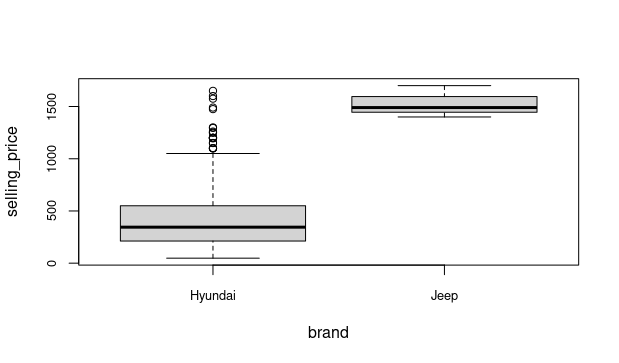
\includegraphics[width=1\textwidth]{unknown.png}
    \item\textbf{Generalized T-test to make comparison between the selected brands:}\\
    To finish, we have to compare the T-test of the selected brands.To do it, we have to use the \texttt{pairwise.t.test()} function that will return what we are expecting. 
    \begin{verbatim}
xx = pairwise.t.test(sub$selling_price, sub$brand, "none")
xx
    \end{verbatim}
The results of the T-test are those belove:
    \begin{verbatim}
    Pairwise comparisons using t tests with pooled SD 

data:  sub$selling_price and sub$brand 

     Hyundai
Jeep 1.2e-11

P value adjustment method: none
    \end{verbatim}
We observe that the $P-value$ between the two selected brands is terse, so the similarities between the two brands in selling prices usually differ significantly.  \\
More specifically,the probability of obtaining a value equal or more extreme than the observed one, assuming that the null hypothesis is true; is the $p-value$ ($1.2\cdot 10^{-11}$).
\end{itemize}

\end{document}
